\begin{titlingpage}
  \thispagestyle{empty}
  \centering
  { \setlength{\baselineskip}{24pt}
    {\Huge \stext{Carbon-12's} \par
      %\textit{for}\par
      \stext{henfaldsprocess}
    }\par
    \stext{(The decay process of carbon-12)}
    \par\vspace*{4\onelineskip}
    \par
    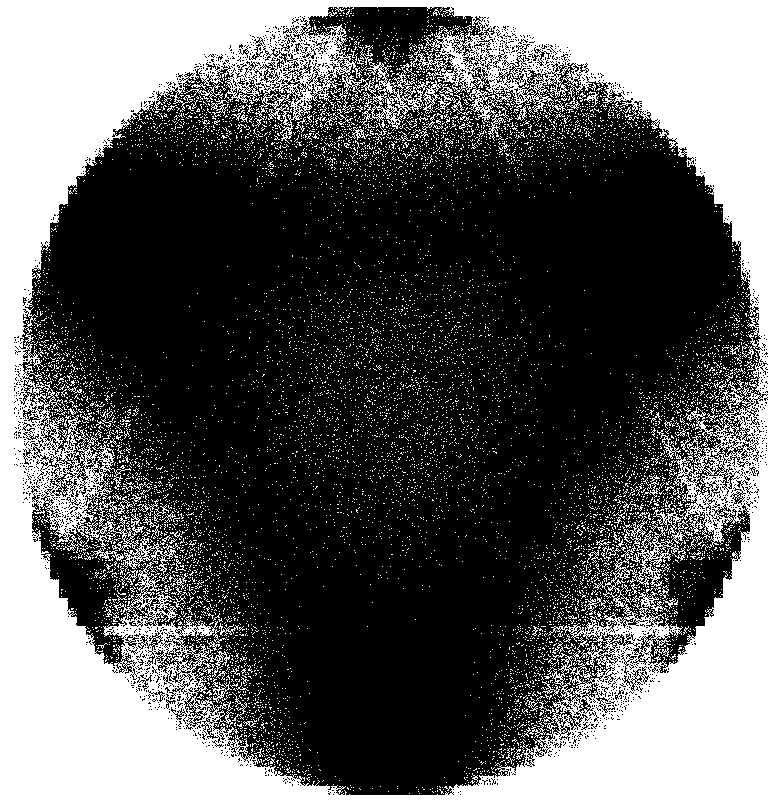
\includegraphics[width=8cm]{forside} 
    \par\vspace*{5\onelineskip}
    \stext{Bachelorprojekt i Fysik}\par
    \large\stext{Michael Kulmback Munch \par 20103561}\par
  }
  \vfill
  \vspace*{2\onelineskip}
  \stext{Vejleder: Hans Fynbo}\hfill
  \stext{1. juli 2013}
  \par\vspace*{2\onelineskip}
  \small
  \stext{Institut for Fysik og Astronomi}\par
  \stext{Aarhus Universitet}
  \enlargethispage{2\onelineskip}

  \newpage
  \thispagestyle{empty} % fjerne evt. sidehoved og -fod
  \small
  % resten af teksten indenfor dette env skal være \small
  \strut\vfill  % pres alt ned i bunden af siden
  \begin{flushleft}
    Institut for Fysik og Astronomi \par
    Aarhus Universitet \par
    Ny Munkegade, Bygning 1520 \par
    DK-8000 Aarhus C \par
    Danmark \par
    \vspace{\onelineskip}
    
    \copyright\ Michael Munch 2013                      \par
    \fxfatal{Not done yet}
    Forsidebilledet er et Dalitzplot.
  \end{flushleft}
\end{titlingpage}